\documentclass[tikz]{standalone}
\usetikzlibrary{positioning}
\usepackage{mathtools}
\newcommand{\red}[1]{\textcolor{red}{#1}}
\newcommand{\blue}[1]{\textcolor{blue}{#1}}
\newcommand{\teal}[1]{\textcolor{teal}{#1}}

\begin{document}
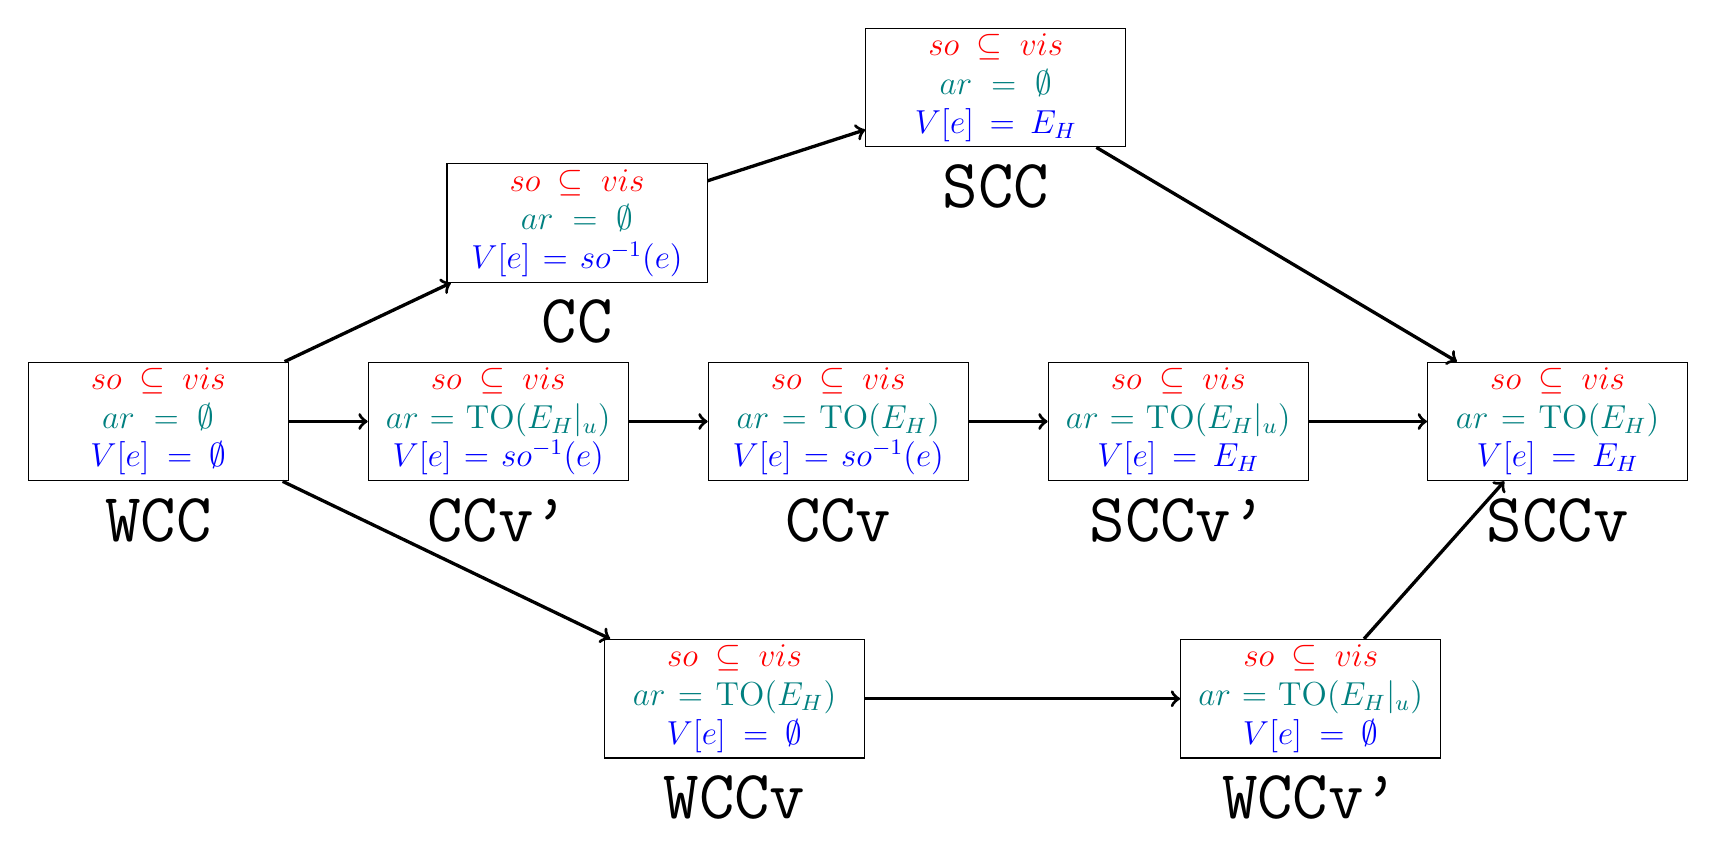
\begin{tikzpicture}
\tikzset{
  lconsistency/.style = {rectangle, fill=white, font=\large, draw, inner sep = 2pt, text width=9em, text centered},
  sconsistency/.style = {rectangle, fill=white, font=\large, draw, inner sep = 2pt, text width=9em, text centered},
  lemma/.style = {rectangle, rounded corners, fill=white, draw=white, line width = 1.5pt, inner sep = 6pt},
  po/.style = {->, very thick},
  cn/.style = {rectangle, fill=white, draw=white,font=\Huge},
}

  \node (wcc) [sconsistency] {%\Large WCC\\
                             \red{$so\subseteq vis$}\\
                             \teal{$ar = \emptyset$}\\
                             \blue{$V[e] = \emptyset$}};
  \node (nwcc) [cn, below = 0.1cm of wcc] {\texttt{WCC}};

  \node (cc) [lconsistency, above right=1.0cm and 2.0cm of wcc] {%\large CC\\
                             \red{$so\subseteq vis$}\\
                             \teal{$ar = \emptyset$}\\
                             \blue{$V[e] = so^{-1}(e)$}};
  \node (ncc) [cn, below = 0.1cm of cc] {\texttt{CC}};

  \node (scc) [sconsistency, above right = 0.2cm and 2.0cm of cc] {%\large SCC\\
                             \red{$so\subseteq vis$}\\
                            \teal{$ar = \emptyset$}\\
                            \blue{$V[e] = E_H$}};
  \node (nscc) [cn, below = 0.1cm of scc] {\texttt{SCC}};

  \node (ccv') [lconsistency, right = 1.0cm of wcc] {%\large CCv'\\
                             \red{$so\subseteq vis$}\\
                             \teal{$ar=\text{TO}(E_H|_u)$}\\
                             \blue{$V[e]=so^{-1}(e)$}};
  \node (nccv') [cn, below = 0.1cm of ccv'] {\texttt{CCv'}};

  \node (ccv) [lconsistency, right = 1.0cm of ccv'] {%\large CCv\\
                             \red{$so\subseteq vis$}\\
                             \teal{$ar=\text{TO}(E_H)$}\\
                             \blue{$V[e]=so^{-1}(e)$}};
  \node (nccv) [cn, below = 0.1cm of ccv] {\texttt{CCv}};

  \node (sccv') [sconsistency,right = 1.0cm of ccv] {%\large SCCv'\\
                             \red{$so\subseteq vis$}\\
                             \teal{$ar = \text{TO}(E_H|_u)$}\\
                             \blue{$V[e] = E_H$}};
  \node (nsccv') [cn, below = 0.1cm of sccv'] {\texttt{SCCv'}};

  \node (sccv) [sconsistency, right = 1.5cm of sccv'] {%\large SCCv\\
                             \red{$so\subseteq vis$}\\
                            \teal{$ar = \text{TO}(E_H)$}\\
                            \blue{$V[e] = E_H$}};
  \node (nsccv) [cn, below = 0.1cm of sccv] {\texttt{SCCv}};

  \node (wccv) [sconsistency, below right=2.0cm and 4.0cm of wcc] {%\large WCCv\\
                             \red{$so\subseteq vis$}\\
                             \teal{$ar = \text{TO}(E_H)$}\\
                             \blue{$V[e] =\emptyset$}};
  \node (nwccv) [cn, below = 0.1cm of wccv] {\texttt{WCCv}};

  \node (wccv') [sconsistency, right = 4.0cm of wccv] {%\large WCCv'\\
                             \red{$so\subseteq vis$}\\
                             \teal{$ar = \text{TO}(E_H|_u)$}\\
                             \blue{$V[e] =\emptyset$}};
  \node (nwccv') [cn, below = 0.1cm of wccv'] {\texttt{WCCv'}};

  \draw [po] (wcc) to (cc);
  \draw [po] (wcc) to (ccv');
  \draw [po] (cc) to (scc);
  \draw [po] (scc) to (sccv);
  \draw [po] (sccv') to (sccv);
  \draw [po] (wcc) to (wccv);
  \draw [po] (wccv) to (wccv');
  \draw [po] (ccv') to (ccv);
  \draw [po] (ccv) to (sccv');
  \draw [po] (wccv') to (sccv);

\end{tikzpicture}
\end{document}
